\label{chap:bfs3}

\alg{Bayesian Forward Search Sparse Sampling}, or \alg{BFS3}, is a method for applying a special kind of tree search to a Bayes-Adaptive Markov Decision Process (BAMDP). \alg{BFS3}, introduced in Section~\ref{sec:bfs3:bfs3} of this Chapter, uses \alg{Forward Search Sparse Sampling} as a subroutine. This application results in a policy with provably efficient sample complexity.

\section{Building blocks}

\alg{BFS3} is built upon the ideas from a few existing algorithms.

\subsection{Sparse Sampling}

\alg{Sparse Sampling}~\cite{kearns99b} works by recursively expanding a full search tree up to a certain depth $d$. At the root, each of the $A$ actions is used for sampling a constant number of times $C$, yielding a set of $A\cdot C$ children. Sparse sampling is then run on each of the children with a recursion depth one less than the root's. Once the tree is fully created, the leaves are each assigned a value of zero. Then, starting at the leaves, the values are backed up and combined via the Bellman equation, defining the parents' values, until the root's value is determined. The total number of nodes visited in this search tree is $(AC)^d$, making the algorithm impractical to run in all but the most trivial of domains.

It is worth noting, however, that \alg{Sparse Sampling} is best known as one of the first reinforcement-learning planning algorithms that can achieve high accuracy with high probability using an amount of computation that is not a function of the size of the state space\footnote{This lack of dependence on the number of states assumes that sampling from the model can be done in constant time. In most real situations there is at least a logarithmic dependency on the number of states just for representing any given state.}. Because of this attractive property, it makes sense to select it or one of its variants as the planner for the infinitely large BAMDP.  \alg{Sparse Sampling} is the basis for a number of Monte-Carlo Tree Search (MCTS) algorithms, which are considerably faster in practice \cite{kocsis06,walsh10,wang05}. \note{ml: "[wel", jta: unfinished comment?}

\alg{Sparse Sampling} is discussed in more detail in Chapter~\ref{sec:relmbbrl}.

\subsection{Forward Search Sparse Sampling}

\alg{Forward Search Sparse Sampling}, or \alg{FSSS}, is a Monte-carlo tree search algorithm used for planning in MDPs. It preferentially expands the search tree through the use of rollouts, and is outlined in Algorithm~\ref{alg:fs3}. Unlike either \alg{Bayesian Sparse Sampling}~\cite{wang05} or \alg{UCT}~\cite{kocsis06}, it retains the attractive guarantees of the original \alg{Sparse Sampling} algorithm. An important property of \alg{FSSS} is that it maintains hard upper and lower bounds, with high probability, on the values for each state and action, and uses those bounds to direct the rollouts; actions are chosen greedily according to the upper bound on the value, and the next state is chosen such that it is the most uncertain of the available candidates (according to the difference in its upper and lower bounds).

%\note{pp: This is a repeat of some text earlier.} \alg{FSSS} will find the action to take from a given state $s_0$, which will be the root of its search tree.  The tree is expanded by running $t$ trajectories, or rollouts, of length $d$. There are theoretically justified ways to choose $t$ and $d$, but in practical applications they are knobs used to balance computational overhead and accuracy. To run a single rollout, the agent will invoke Algorithm~\ref{alg:fs3-rollout}, $\mbox{FSSS-Rollout}(s_0, d, 0, M)$.
%, $T$ times. 
The values $U_d(s)$ and $L_d(s)$ are the upper and lower bounds on the value of the node for state $s$ at depth $d$, respectively. Each time a rollout is performed, the tree will be expanded. After at most $(AC)^d$ rollouts are finished (but often less in practice), \alg{FSSS} will have expanded the tree as much as is possibly useful, and will agree with the action chosen by \alg{Sparse Sampling}.

\alg{FSSS} is discussed in more detail in Chapter~\ref{sec:relmbbrl}.

\section{Bayesian Forward Search Sparse Sampling}

\label{sec:bfs3:bfs3}

\begin{algorithm}[tb]
	\caption{$\mbox{BFS3}(s, h, d, C, t, \phi)$}
	\label{alg:bfs3}
	\KwIn{state $s$, history $h$, depth $d$, branching factor $C$, \#trajectories $t$, MDP prior $\phi$}
	\KwOut{action to take in state $s$}
	\If {$\langle s,h\rangle \in K$} {
		\Return $\pi(\langle s,h \rangle)$
	}
	\ForEach {$a \in A$} {
		$q(a) \leftarrow 0$\\
		\For {$C$ times} {
			$\langle s', h'\rangle , r \sim {T\mbox{-}R}_\phi(\langle s,h\rangle, a)$\\
			$q(a) \leftarrow q(a) + \frac 1 C \left[r+ \gamma FSSS(\langle s', h'\rangle, d, C, t, M_\phi)\right]$
		}
	}
	$K \leftarrow K \bigcup \{\langle s,h\rangle\}$\\
	$\pi(\langle s,h\rangle) \leftarrow \argmax_a q(a)$\\
	\Return $\pi(\langle s,h\rangle)$\\
\end{algorithm}


\alg{BFS3} is the application of \alg{FSSS} to a Bayes-adaptive MDP, or BAMDP. The BAMDP is defined by the MDP prior~$\phi(M)$, and the joint transition and reward function ${T\mbox{-}R}_\phi$ is constructed such that
\begin{eqnarray*}
P(\langle s', h + (s,a,s',r)\rangle, r | \langle s, h\rangle, a) &=& \int_M P(s', r | s, a, M)\phi(M|h) dM.
\end{eqnarray*}

Here, the BAMDP's state-space is the set of belief-states that include the history of all transitions seen so far. Because of how the BAMDP's transition function is constructed, each possible next-state's history includes the transition from the previous state to the next state.

BAMDPs, their construction, and their relation to Bayes-optimality are discussed in detail in Chapter~\ref{sec:intro}.

Since, with \alg{FSSS}, the next belief-states are only sampled and their likelihoods are never calculated, a simple generative process can be used:
\begin{eqnarray}
M &\sim& \phi|h \label{eq:oracle1}\\
s', r &\sim& T_M(s,a), R_M(s,a).\label{eq:oracle2}
\end{eqnarray}

This process is used whenever \alg{BFS3} or its subroutine \alg{FSSS} sample a next-state and reward. The algorithm never holds on to an individual MDP after a single transition has been sampled from it. Also, note that whenever \alg{FSSS} does a Bellman backup, that backup is done for a belief-state (since \alg{FSSS} is acting on the BAMDP).

First, an MDP $M$ is sampled from the posterior $\phi|h$. Once it is sampled, then the next state and reward are sampled from $M$. Sometimes this posterior sampling can be computationally expensive, since inference is generally a hard probelm. The \alg{BFS3} algorithm can only work effectively if this step is fast. Fast posterior sampling is possible with many priors, including the very simple \prior{FDM}, but also more structured priors can be used with efficient inference --- all the priors used with \alg{BFS3} in Chapter~\ref{sec:experiments} have efficient posterior inference.

To reconstruct the resulting belief-state, we pack the resulting concrete state $s'$ with the new history made by augmenting $h$ with $(s, a, s', r)$, resulting in a transition from belief-state $\langle s, h\rangle$ to $\langle s', h + (s,a,s',r)\rangle$. \note{jta: your annotation suggested I change this to "resulting in a transition belief-states $<s,h>$ and $<s',h+....$", and I don't get it} In many cases, the history $h$ can be summarized by a more compact sufficient statistic. For instance, with discrete-state and -action MDPs, only a histogram of next-states needs to be kept for each state-action pair, and the exact sequence that these transitions happened in is irrelevant.

Figure~\ref{fig:bfs3} illustrates \alg{BFS3}'s process for each belief-state visited by the agent. In future steps through the environment, the agent may find itself in one of the reachable belief-states in the search tree --- all of the reachable belief-states represent one possible concrete state and history that, with some probability, may be the root of \alg{BFS3}'s search tree in some future situation. 

\subsection{Algorithm}

The \alg{BFS3} process is detailed in Algorithm~\ref{alg:bfs3}, which references Algorithm~\ref{alg:fs3} in Chapter~\ref{sec:relatad}. Every time the agent arrives in a new belief-state $\langle s, h\rangle$, it simulates each action $C$ times, to get a set of $C \times A$ next belief-states and rewards. Then, \alg{FSSS} is used to find the upper bound on the value of each of the next belief-states. Once their optimistic values are found, \alg{BFS3} will average all the sums of the discounted values and rewards together to get an estimate of the Bayes-expected value of taking that action, and choose the action that maximizes this quantity.

All histories should only take into account the first $B$ transitions from a given state-action pair, where $B$ is the number of transitions required to have accurate posterior samples for any particular state-action. The exact value for $B$ is tied to the \bed-learnable condition in Section~\ref{sec:bfs3:pac-bamdp-informal}, condition~\ref{theorem:cond-acc}.

Putting a limit on the number of transitions to remember for a particular state-action pair does two important things. First, it means it is possible for the agent to end up in the same effective belief-state more than once\footnote{Normally, an agent would never experience the same belief-state twice, because every step it takes grows the history by one transition.}. This allows \alg{BFS3} to reuse past decisions and puts a bound on the number of decisions that can be made, saving computation time. Second, it aids in the PAC-BAMDP proof, since the number of random events that need to succeed is bounded.

\begin{figure}
\vskip 0.2in
\begin{center}
\centerline{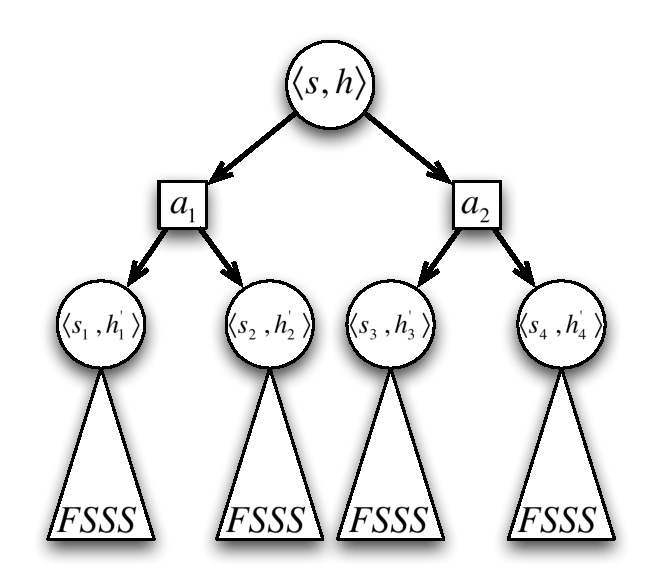
\includegraphics[scale=0.5]{figures/bfs3}}
\caption{
%{\bf Left:} the search tree when the agent is at state $s_0$ with no further observations. {\bf Right:} the agent has taken a single step in the world by performing action $a_1$, resulting in a transition to state $s_2$. White nodes indicate hypotheticals that may or may not happen. Grayed nodes indicate things that have been observed. Blackened nodes indicate data that is no longer pertinent and can be thrown out.
\alg{BFS3} samples next-belief-states for each action $C$ times, and then runs \alg{FSSS} on the resulting belief state, using the BAMDP as a generative model. Every node that is the same distance from the root represents one of the possible worlds that the agent may experience, each with a different history and MDP posterior.
}
\label{fig:bfs3}
\end{center}
\vskip -0.2in
\end{figure} 

\subsection{BFS3 is PAC-BAMDP}
\label{sec:bfs3:pac-bamdp-informal}

If certain reasonable prerequisites are satisfied, then with high probability, \alg{BFS3} will choose actions that are approximately Bayes-optimal except for a small number of times.
\begin{thm}
If, with MDP prior $\phi$,
\begin{enumerate}
\item
\label{theorem:cond-acc} 
for any state-action pair $(s,a)$, a history $h$ that is made of observations sampled from $m_0$ and contains at least $B$ examples of transitions from $(s, a)$,
$$\left|T_{m_0}(s'|s,a) - T_{\phi|h}(s'|s,a)\right| \leq \epsilon_l,$$
with probability at least $1-\delta_l$,
where $T_{\phi}(s'|s,a) =\int_m \phi(m|h) T_m(s'|s,a) dm$ is the posterior transition likelihood,
\item
\label{theorem:cond-fsss}
\alg{FSSS}, given the true MDP $m_0$, $T$ trajectories, searching up to depth $D$, with a branching factor of $C$, can provide $\epsilon_p$-accurate value estimates with probability at least $1-\delta_p$, and 
\end{enumerate}
then, with probability at least $1-\delta$, \alg{BFS3} will behave $\epsilon$-Bayes-optimally for all but a number of steps that is polynomial with the number of states, the number of actions, $\gamma$, $\epsilon$, $\delta$, and $B$, where
\begin{eqnarray}
\epsilon_l &=&,\\
\delta_l &=&,\\
\epsilon_p &=&,\\
\delta_p &=&.
\end{eqnarray}
\end{thm}

Prerequisite~\ref{theorem:cond-acc} can be interpreted as the expected posterior likelihood of a transition being $\epsilon_l$-close to the true likelihood of that transition.

\begin{proofsketch}

First, we will show that there is a BAMDP, constructed from the prior $\phi$, whose optimal policy is the Bayes-optimal policy for $m_0\sim \phi$. Then, we will show that \alg{BFS3}, acting in the BAMDP, will satisfy the three criteria required for PAC-MDP behavior~\cite{kakade03,lihong09pacmdp} in that BAMDP\footnote{PAC-MDP behavior in the BAMDP implies near Bayes-optimal behavior in the learning setting.}.
These criteria are: \begin{inparaenum} \item accuracy, \item bounded discoveries, and \item optimism. \end{inparaenum}

First, because of Prerequisite~\ref{theorem:cond-acc} in our theorem statement, we know that once we have received $B$ examples of transitions from a state-action pair $(s,a)$, our estimate of the next-state distribution for that pair will be accurate.  (This condition need not hold for degenerate priors, but it appears to hold quite broadly.)

Second, since we forget all additional transitions from state-action pairs for which we have seen $B$ examples, the number of possible state-histories that an agent can observe is bounded.  Specifically, each time a transition from some state-action $(s,a)$ is observed, either no change will be made to the state-action's histogram (it already sums to $B$), or exactly one entry in the histogram will be incremented by $1$.  Since the histogram can be changed at most $B$ times, the total number of histories possible for an agent over the course of a single experiment is $B \cdot S \cdot A$ ($B$ histories for each state-action pair).

A discovery event, or one that potentially changes the MDP posterior, is an event that results in a change to the history. There are $B \cdot S \cdot A$ discoveries possible, since other transitions will be forgotten.

Third, $\mathbf{FSSS}(s',d,C,t,M_\phi)$ is guaranteed to have an optimistic value estimate for belief-state $s'$ as $t$ (the number of trajectories), our bounded resource, grows smaller. We also know that, from Prerequisite~\ref{theorem:cond-fsss} of the theorem, $t$ is sufficient to find accurate estimates of $s'$ if all states in $s'$'s subtree have converged next-state posteriors. Simply put, if $s'$'s subtree has no unknown state-action pairs, then \alg{FSSS}'s estimate of that state's value will be accurate.  As a result, if \alg{FSSS}'s estimate of a state's value is inaccurate, there must be something to learn about in $s'$'s subtree. \alg{FSSS} guarantees that this inaccuracy will be optimistic.

Also possible is that the value estimate of $s'$ is accurate \emph{and} there are unknown states in its subtree. In this case, the agent can decide whether or not to visit that state fully informed of its value, and can take a Bayes-optimal action.

The PAC-MDP criteria direct the agent to areas of either high value or high uncertainty, managing the exploration/exploitation tradeoff. Because the agent will only go to areas of high uncertainty over areas of high reward a bounded number of times that grows linearly with the number of possible discovery events, we bound the number of sub-optimal steps taken over the lifetime of the agent.
\end{proofsketch}


\section{Proof of PAC-BAMDP}

This section presents the detailed argument that \alg{BFS3} is near
Bayes-optimal.


\subsection{Terms}
\begin{itemize}
\item $B$ is the maximum number of transitions that will be observed from any particular state-action pair. All subsequent transitions will not be recorded.
\item The history $h\in H$ is the collection of the first $B$ observed transitions $(s,a)\rightarrow s'$.
\item $\phi$ is the MDP prior. $\phi|h$ is the MDP posterior.
\item $m_0$ is the unknown true MDP.
\item $T_m(s'|s,a)$ is the probability of going from $s$ to $s'$ when performing action $a$ in some MDP~$m$.
\item $R_m(s,a)$ is the known reward function of MDP $m$.
\item The \emph{experiment} is the possibly infinite sequence of $o_{t+1} = (s_t,a_t,s_{t+1},r_t)$ observations made by the agent, each with the likelihood
$$P(o_{t+1}|o_1,o_2,...,o_{t+1}) = T_{m_0}(s_{t+1}|s_t,a_t)\mathbb{1}(r_t = R_{m_0}(s_t,a_t)).$$
That is, the sequence of observations making up the experiment comes from $m_0$.
\item $T_{\phi|h}(s'|s,a)=\int_m \phi(m|h)T_m(s'|s,a) dm$ is the posterior transition likelihood, integrated over all possible MDPs.
\item $V_m(s)$ is the true value of state $s$ according to MDP $m$.
\item $\mbox{FSSS}_m(s, X)$ is the value of state $s$ estimated by \alg{ FSSS} when using $s$ as a root, $m$ as an oracle (that samples next-states given a state-action pair), and with computational resource bounds represented by $X$. In this context, $X$ is the number of trajectories, the branching factor, and the search depth that \alg{FSSS} uses to perform roll-outs.
\end{itemize}

\subsection{Assumptions}
\begin{enumerate}
\item \label{fsss-acc} The {\bf planning assumption}: For any $s$, with probability at least\ $1-\delta_p$, 
\begin{eqnarray}
|\mbox{FSSS}_{m_0}(s, X)-V_{m_0}(s)| &\leq& \epsilon_p.
\end{eqnarray}
In other words, \alg{FSSS} will estimate values accurately if it is given the true model.
\item \label{sa-bound} The {\bf accuracy assumption}: For some state-action pair $(s,a)$, if $h$ includes $B$ samples from $T_{m_0}(s'|s,a)$, then with probability at least $1-\delta_l$,
\begin{eqnarray}
\forall_{s'}~|T_{\phi|h}(s'|s,a) - T_{m_0}(s'|s,a)| \leq \epsilon_l.
\end{eqnarray}
As a result, if $B$ examples of each of the $S\cdot A$ state-action pairs are observed, with probability at least $1-\delta_l S A$, all transition probability deviations are bounded by $\epsilon_l$.

\item The {\bf MCTS simulation conjecture}, described in Section~\ref{mcts-conj}.
\end{enumerate}



\subsection{MCTS simulation conjecture}
\label{mcts-conj}

Let an MCTS algorithm $\mathcal{A}_m(s,B)$ be an estimator of the value of state $s$ in MDP $m$, bounded by computational resources $B$, whose sole source of stochasticity comes from using $m$ as a generator of $s'\sim s,a|m$. \alg{FSSS} and \alg{UCT}~\cite{kocsis06} both fall into this category; their resources are the number of roll-outs and maximum search depth.

Intuitively, we conjecture that if $\mathcal{A}$ can reliably find accurate values for states in one MDP, then it can also reliably find accurate values for the MDP when using an approximate second MDP as its next-state generator.

If,
\begin{enumerate}
\item \label{mcts-bound} for all $s,a,s'$, $|T_{m_a}(s'|s,a) - T_{m_b}(s'|s,a)| \leq \epsilon_l$,
\item \label{mcts-good} for all $s$, with probability at least $1-\delta_p$, $|\mathcal{A}_{m_a}(s,X)-V_{m_a}(s)|\leq \epsilon_p$,
\end{enumerate}
then for all $s$, with probability at least $1-f_\delta(\delta_p)$,
\begin{eqnarray}
|\mathcal{A}_{m_b}(s,X)-V_{m_a}(s)|\leq f_\epsilon(\epsilon_l, \epsilon_c),
\end{eqnarray}
where
\begin{eqnarray}
1/f_\delta(\delta_p)&=&\mbox{poly}(1/(1-\epsilon_l),1/\delta_c,1/\epsilon_c,m_a,B)\\
f_\epsilon(\epsilon_l, \epsilon_p)&=&\mbox{poly}(1/(1-\epsilon_l),1/\delta_c,1/\epsilon_c,m_a,B).
\end{eqnarray}


%\subsubsection{Note on $C \cdot A$}
%The probability $1-\delta_{p}/(CA)$ is used because, for each step, \alg{BFS3} will invoke \alg{FSSS} $C \cdot A$ times, or $C$ times for each action.  This choice was made to ensure that all next states get enough resources to ensure accuracy when their dynamics are known. We use the union bound to say, with probability  $1-\delta_p$, \emph{all} such next states have accurate estimates.

\note{ml: [it would be nice to have a note explaining the status of this conjecture.  My gut feeling is that it is false.  But perhaps some version of it could hold.  But, maybe a short section explaining what you've learned in trying to prove this conjecture would be worthwhile.] jta: it is definitely false, in general (I can construct a degenerate counter-example.)}

\subsection{PAC-MDP behavior in the BAMDP}

Let
\begin{itemize}
\item the BAMDP be $m_{\phi|h}$,
\item the set of all possible histories be $H$,
\item the state space of the BAMDP be the set of belief-states $S_\phi = S \times H$, and
\item the action space of the BAMDP be the same as the regular MDP.
\end{itemize}

\alg{BFS3} limits $H$ to contain only histories with at most $B$ examples of transitions from any state-action pair. That is, when the agent observes the $B_{\mbox{\footnotesize{th}}}$ transition from state $s$ and action $a$, it shall never again update its history when making a transition from that state with that action. This forgetfulness causes the set $H$ to be finite without sacrificing accuracy, due to Assumption~\ref{theorem:cond-acc}.

In a discrete state and action MDP, the history $h\in H$ may be summarized by a set of histograms, one for each state-action pair. Since we ignore all transitions from any state-action pair after the $B_{\mbox{\footnotesize{th}}}$ transition from that state-action pair, we know that the sum of all entries in all histograms cannot exceed $S\cdot A \cdot B$.

Since, whenever the history \emph{is} updated, a single entry for a single histogram will be incremented by $1$, we can infer that a sequence of at most $S\cdot A \cdot B$ unique histories can possibly be experienced by an agent over the course of a single experiment.

The agent can also visit at most $S$ true states (all of them). Since there are $S$ true states and $S\cdot A \cdot B$ possible histories, the number of belief-states that an agent can visit, in a single experiment, is $M = S^2\cdot A \cdot B$.

Our strategy will be to say that, for each of these at most $M$ possible belief-states visited by the agent, the agent will either choose an action that is approximately optimal in the BAMDP (and therefore approximately Bayes-optimal in the true MDP), or exploratory in the BAMDP (with no guarantees about how good this action is in the true MDP).

We say that an agent is near Bayes-optimal if we can limit the number of exploratory actions taken to a polynomial of the domain parameters.

To show PAC-MDP behavior in the BAMDP (and, therefore, near Bayes-optimal behavior), we need to show that three conditions hold~\cite{lihong09pacmdp}:
\begin{enumerate}
\item \label{pacmdp-disc} bounded discoveries,
\item \label{pacmdp-acc} accuracy, and
\item \label{pacmdp-opt} optimism.
\end{enumerate}

To understand these criteria and how they connect PAC-MDP behavior in the BAMDP to near Bayes-optimal behavior in the true MDP, we need to define the concept of \emph{known} and \emph{unknown} \emph{states} in $m_0$ and  \emph{known} and \emph{unknown} \emph{belief-states} in $m_\phi$.

A \emph{state} $s$ is considered known if the history $h$ contains $B$ examples of transitions from $s$ for each action $a\in A$.

A \emph{belief-state} $\langle s, h \rangle$ is considered known if \alg{FSSS}'s estimate of its value is accurate.

Figure~\ref{fig:bfs3tree} illustrates how unknown states in a belief-state's \alg{FSSS} subtree may cause a belief-state's estimate to be inaccurate. Because of Prerequisite~\ref{fsss-acc}, the planning assumption, we know that if there are no unknown states in a belief-state's subtree, then the belief-state's estimate will be accurate, and we can consider the belief-state to be known.

It is possible for a belief-state to be known if there are unknown states in its subtree; in the limit of computation, \alg{FSSS} will be accurate for all belief-states. But, it is not possible for all states in the belief-state's subtree to be known if the belief-state is not known.

As a result, an unknown belief-state indicates an unknown state that is at most $D+1$ steps away, where $D$ is the search depth given to \alg{FSSS} (which starts planning from $1$ step in the future). Since unknown belief-states always have optimistic estimates when they are evaluated with \alg{FSSS}, the agent is pulled towards unknown states.

\begin{figure}
\vskip 0.2in
\begin{center}
\centerline{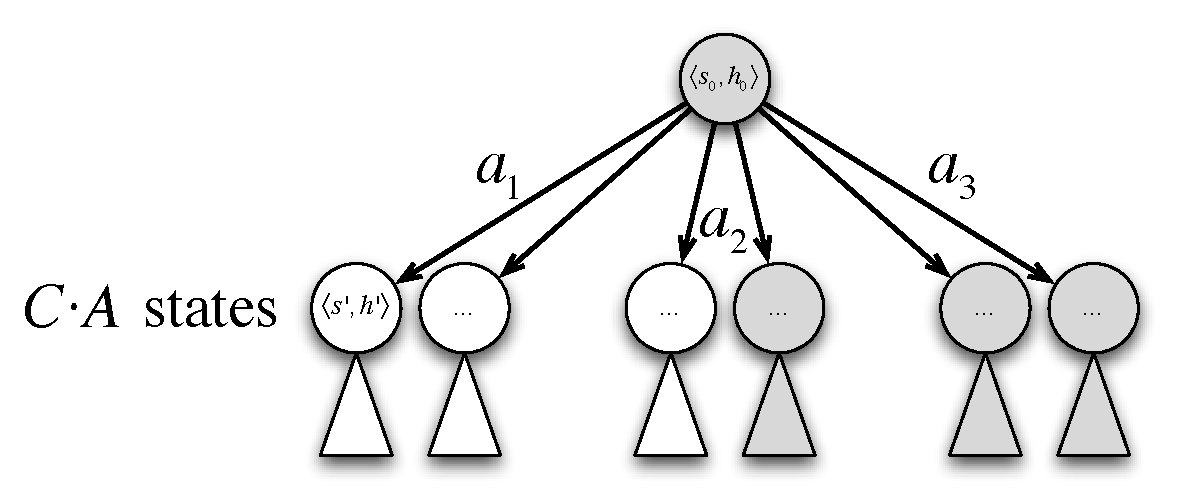
\includegraphics[scale=0.5]{figures/bfs3tree}}
\caption{
\alg{BFS3} will run \alg{FSSS} on each of the $C\cdot A$ next belief-states, $\langle s', h' \rangle$ and its peers. Triangles below belief-states represent search trees explored by \alg{FSSS}. A greyed search tree indicates that some of the true states visited in that search tree are unknown, and the value estimate may be inaccurate. Because we are using \alg{FSSS}, an inaccurate estimate is guaranteed to be optimistic, and can bubble up to the root.
}
\label{fig:bfs3tree}
\end{center}
\vskip -0.2in
\end{figure} 

\subsubsection{Satisfying the PAC-MDP criteria}

\alg{BFS3} is PAC-MDP for the belief-state MDP because it satisfies the 3 criteria.

Condition~\ref{pacmdp-disc} holds because if the agent reaches an unknown belief state (one with an inaccurate, optimistic value), it must be because there is an unknown state-action pair beneath it in the tree \emph{and} this node will be reached by the current policy with high probability.  (Quantifying this claim \note{ml: [I'm afraid you need to do it.  it's just a sketch otherwise and you are claiming this result as one of your principal contributions]} involves an argument that closely parallels the ``explore or exploit'' lemma from PAC-MDP theory.)  Note that when an unknown state-action pair is reached, it moves closer to being known.  In fact, an agent can only do this update $S\cdot A \cdot B$ times, so, the number of discoveries is bounded.

% Condition~\ref{pacmdp-disc} holds because a discovery is an event that updates the posterior, or changes the history. Since an agent can only do this update $S\cdot A \cdot N$ times, the number of discoveries is bounded by $S\cdot A \cdot N$.

Condition~\ref{pacmdp-acc} holds because of Prerequisite~\ref{sa-bound} (the accuracy assumption). Once we have $B$ examples of a state-action pair, we have an accurate estimate of the next-state distribution for that pair. Once we have $B$ examples of all state-action pairs, we have an accurate estimate of the entire MDP.

%Condition~\ref{pacmdp-opt} holds because of the nature of \alg{FSSS}. We know that \alg{FSSS} will never be pessimistic about a state's value~\cite{walsh10}. We will allow any uncertainty in a belief-state's value (that is, it can possibly run into a state-action pair for which $N$ samples have \emph{not} been observed) to cause \alg{FSSS} to be inaccurate. And, if it is not accurate, \alg{FSSS} must be optimistic. In this sense, uncertainty will draw the agent towards unknown states.

Condition~\ref{pacmdp-opt} holds because of our definition of known and unknown belief-states and the behavior of \alg{FSSS}. Known belief-states have accurate values, and unknown belief-states have optimistic values. No belief-state ever has a pessimistic value.

\subsection{How accurate, and how likely?}

We have shown that \alg{BFS3} is near Bayes-optimal, meaning, with high probability, it will be accurate for all but a small number of steps. This section details how accurate \alg{BFS3} is and with what probability it achieves this accuracy.

\subsubsection{Bayes-optimal behavior for a converged posterior}
\label{sec-conv}
We declare the posterior to be converged if, for each $s,a$, our history $h$ includes $B$ examples of a transition from $s,a$.

\begin{lemma}
If,
\begin{itemize}
\item
for a given state-action pair $(s,a)$, $\forall_{s'} |T_{m_0}(s'|s,a) - T_{\phi|h}(s'|s,a)| \leq \epsilon_l$ with probability at least $1-\delta_l$,
\item
for a given state $s$, $|\mbox{FSSS}(s,X,\phi|h)-V_{\phi|H}(s)| \leq \epsilon_p$ with probability at least $1-\delta_p$,
\end{itemize}
then,
\begin{eqnarray}
\forall_s \ |\mbox{FSSS}(s,X,\phi|h) - V_{m_0}(s)| &\leq& f_\epsilon(\epsilon_l,\epsilon_p),
\end{eqnarray}
with probability at least $1-S A \delta_l - C A f_\delta(\delta_p)$.
\end{lemma}
\begin{proof}
The probability that the posterior is $\epsilon_l$-close for a single state-action pair is at least $1-\delta_l$, according to  Prerequisite~\ref{theorem:cond-acc}. Applying the union bound then tells us that the probability that all $S \cdot A$ state-action pairs have an $\epsilon_l$-accurate posterior is at least $1- SA \delta_l$.

Let $m_0$ and $\phi|h$ take the place of $m_a$ and $m_b$ in the MCTS simulation conjecture.
By Prerequisite~\ref{sa-bound}, we have Condition~\ref{mcts-bound} for the MCTS simulation conjecture. 
By Prerequisite~\ref{fsss-acc}, we have Condition~\ref{mcts-good} for the MCTS simulation conjecture.

For each step in the environment, \alg{BFS3} runs \alg{FSSS} $C$ times for each action, resulting in $C\cdot A$ executions of \alg{FSSS}. We can use the union bound to put a lower bound on the likelihood that they are all $f_\epsilon(\epsilon_l, \epsilon_p)$-accurate of at least $1-CAf_\delta(\delta_{p})$, assuming that all transition probabilities in $\phi|h$ are $\epsilon_l$-accurate.

We can use the union bound again to assert that the probability that all $S\cdot A$ posterior transition likelihoods are $\epsilon_l$-accurate, and that all $C\cdot A$ executions of \alg{FSSS} are $f_\epsilon(\epsilon_l,\epsilon_p)$-accurate, at the same time, is $1 - SA \delta_l-CAf_\delta(\delta_p)$.
\end{proof}

Now that the accuracy and likelihoods for the calls out to \alg{FSSS} have been estabilished, we can see how they affect the decision made by \alg{BFS3}.

\begin{lemma}
If \alg{FSSS} makes $f_\epsilon(\epsilon_l,\epsilon_p)$-accurate estimates for all states, then \alg{BFS3} will make an $(\epsilon_e+f_\epsilon(\epsilon_l,\epsilon_p))$-optimal decision with probability at least $1-e^{-\epsilon_e^2 C / {\Vmax^2}}$.
\end{lemma}

\begin{proof}

The estimate for the value of taking action $a$ from the root state $s_0$ is calculated as
\begin{equation}
\hat Q(s_0, a) = R(s_0,a) + \gamma \frac 1 C \sum_{i=1}^C \mbox{FSSS}_{\phi|h}(s_i, B).
\end{equation}

Let the Monte~Carlo estimate of $Q(s_0,a)$, using the true value for all next states, be
\begin{equation}
\tilde Q(s_0, a) = R(s_0,a) + \gamma \frac 1 C \sum_{i=1}^C V_{m_0}(s_i).
\end{equation}

From the Bellman equation, we know that
\begin{equation}
Q_{m_0}(s_0, a) = R(s_0,a) + \gamma \sum_{s_i} P_{m_0}(s_i|s,a) V_{m_0}(s_i).
\end{equation}

First, let's bound the difference between $\hat Q(s_0, a)$ and $\tilde Q(s_0, a)$.
\begin{eqnarray}
\nonumber |\hat Q(s_0, a) - \tilde Q(s_0, a)| &=& \left|\gamma \frac 1 C \sum_{i=1}^C \mbox{FSSS}_{\phi|h}(s_i, B) - \gamma \frac 1 C \sum_{i=1}^C V_{m_0}(s_i)\right|\\
\nonumber &=& \left|\gamma \frac 1 C \sum_{i=1}^C \left(\mbox{FSSS}_{\phi|h}(s_i, B) -  V_{m_0}(s_i)\right)\right|\\
\nonumber &\leq& \gamma \frac 1 C \sum_{i=1}^C \left|\mbox{FSSS}_{\phi|h}(s_i, B) -  V_{m_0}(s_i)\right|\\
\nonumber &\leq& \gamma \frac 1 C \sum_{i=1}^C f_\epsilon(\epsilon_l, \epsilon_p)\\
 &\leq& f_\epsilon(\epsilon_l, \epsilon_p).
\end{eqnarray}

Second, let's bound the difference between $\tilde Q(s_0, a)$ and $Q_{m_0}(s_0, a)$.
\begin{eqnarray}
\nonumber |Q_{m_0}(s_0, a) - \tilde Q(s_0, a)| &=& \left|\gamma \sum_{s_i} T_{m_0}(s_i|s,a)V_{m_0}(s_i) - \gamma \frac 1 C \sum_{i=1}^C V_{m_0}(s_i)\right|\\
\nonumber &=& \gamma \left|\sum_{s_i} T_{m_0}(s_i|s,a)V_{m_0}(s_i) - \frac 1 C \sum_{i=1}^C V_{m_0}(s_i)\right|\\
 &\leq& \epsilon_e,
\end{eqnarray}
with probability at least $1-e^{-\epsilon_e^2 C / {\Vmax^2}}$~\cite{kearns99b}.

This expression bounds the error in the estimated Q-values:
\begin{eqnarray}
\nonumber |\hat Q(s_0, a) - Q_{m_0}(s_0, a)| &=& |\hat Q(s_0, a) - \tilde Q(s_0, a) + \tilde Q(s_0, a) - Q_{m_0}(s_0, a)|\\
\nonumber &\leq& |\hat Q(s_0, a) - \tilde Q(s_0, a)| + |\tilde Q(s_0, a) - Q_{m_0}(s_0, a)|\\
 &\leq& f_\epsilon(\epsilon_l, \epsilon_p)+\epsilon_e,
\end{eqnarray}

with probability at least $1 - e^{-\epsilon_e^2 C / {\Vmax^2}}$.

\end{proof}

Once the model has converged, every time the agent takes a step from some state $s_0$ it remembers what action it took, and will take that action in the future. 

Let $\epsilon_c = f_\epsilon(\epsilon_l, \epsilon_p)+\epsilon_e$, and $\delta_c = S A \delta_l + C A f_\delta(\delta_p) + S(e^{-\epsilon_e^2 C / {\Vmax^2}})$.

\begin{lemma}
\label{sec:bfs3:lemma:converged}
Once at least $B$ examples of transitions from each state-action pair have been observed, the likelihood of \alg{BFS3} choosing an $\epsilon_c$-optimal action for each of the $S$ possible states is no less than $1-\delta_c$.
\end{lemma}
\begin{proof}
Proof follows immediately from the union bound.
\end{proof}

\subsection{Bayes-optimal behavior for an unconverged posterior}

Since the agent will not update the history $h$ on a transition from $s,a$ when transitions $s,a$ have been observed $B$ times in the past, we know there are only $S \cdot A \cdot B$ different histories possible over the course of a single experiment.

Given a particular history $h$ and state $s$ that has been experienced before, \alg{BFS3} will choose the same action as last time, limiting the total amount of computation possible; in addition, the total number of times \alg{BFS3} has to succeed is limited at $M = S^2 A B$, or the number of states times the number of possible histories.

In Sections~\ref{sec:inf}~and~\ref{sec:fin}, we set conditions for \alg{BFS3} to choose either an exploratory action or an optimal action for each of these $M$ possible events.

On a given step, \alg{BFS3} will run \alg{FSSS} for each of $A$ possible actions and, for each action, $C$ possible next-states.


\subsubsection{In the limit of infinite computation}
\label{sec:inf}

We will briefly examine the behavior of \alg{BFS3} as the number of trajectories $t$, the branching factor $C$, and the search depth $D$ all approach infinity.

\begin{lemma}
As $t\rightarrow \infty$, \alg{BFS3} will make $\epsilon_\infty$-Bayes-optimal decisions for all steps with probability $1-\delta_\infty$, where
\begin{eqnarray}
\epsilon_\infty &=& \frac {\epsilon_e(1-\gamma^{D+1})} {1-\gamma}+\gamma^D\Vmax,\\
\delta_\infty &=& M(CA)^D e^{-\epsilon_e^2C/\Vmax^2}.
\end{eqnarray}
\end{lemma}
\begin{proof}
Each of the next-state possibilities will be fully explored and FSSS will agree with Sparse Sampling, giving an error of no more than 
$$\epsilon_\infty = \frac {\epsilon_e(1-\gamma^{D+1})} {1-\gamma}+\gamma^D\Vmax,$$
with probability at least $1-(C\cdot A)^D e^{-\epsilon_e^2C/\Vmax^2}$, where $D$ is the maximum search depth. Recall that $M = S^2 A B$ is the maximum number of decisions that \alg{BFS3} will have to make. Let $\delta_\infty/M=(C A)^De^{-\epsilon_e^2C/\Vmax^2}$; the agent will then be able to pick an $\epsilon_\infty$-optimal action for each of the $M$ events with probability  at least $1-\delta_\infty$.
\end{proof}


\subsubsection{Limited computation}
\label{sec:fin}

When computation is limited, we have to rely on optimistic estimates of Q-values in the BAMDP to draw the agent towards unknown belief-states that are potentially optimal.

In cases where there is limited computation and all states in the subtree have converged according to Prerequisite~\ref{sa-bound}, we are guaranteed to act $\epsilon_f$-optimal with probability  at least $1 - \delta_f/M$, according to Lemma~\ref{sec:bfs3:lemma:converged}, where
$$\epsilon_f = f_\epsilon(\epsilon_l, \epsilon_p)+\epsilon_e$$
and
$$\delta_f/M = f_\delta(\delta_{p}) + e^{-\epsilon_e^2 C / {\Vmax^2}}.$$

In cases with limited computation and when there are states in the subtree that are not converged, we are guaranteed to have an $\epsilon_f$-\emph{optimistic} estimate with probability  at least $1-\delta_f/M$. This is true because of the guarantees provided by \alg{FSSS}.

An action $a$'s estimate is $\epsilon$-optimistic if
$$\hat Q(s, a) \geq Q_{m_0}(s, a) - \epsilon.$$

Note that an $\epsilon$-accurate estimate is also $\epsilon$-optimistic.

Since for each of the $M$ events we have an $\epsilon_f$-optimistic estimate with probability  $1-\delta_f/M$, we will have an $\epsilon_f$-optimistic estimate for each event simultaneously with probability  $1-\delta_f$, by the union bound.

%We can now lean on the PAC-MDP proof for $\epsilon_f$-optimal behavior in the belief MDP with probability  $1-\delta_f$ for all but a polynomial number of steps.

%If we take an action whose estimate is $\epsilon_f$-optimistic but not $\epsilon_f$-optimal, that means that there must be something worth learning (in that if we knew it, it has the potential to change our estimate) in the next $D$ steps.

%
\ifperchapterbib%
For the convenience of the reader, a list of references is provided at the end of each chapter (where applicable).
\ifendbib%
%A bibliography containing all cited references is included at the \hyperref[sec:bibliography]{end of the dissertation}.
\else\fi% end ifendbib
%\cbend%
\else\fi% end ifperchapterbib
